%-----------------------------------------------------------------------------
%
%               Template for sigplanconf LaTeX Class
%
% Name:         sigplanconf-template.tex
%
% Purpose:      A template for sigplanconf.cls, which is a LaTeX 2e class
%               file for SIGPLAN conference proceedings.
%
% Guide:        Refer to "Author's Guide to the ACM SIGPLAN Class,"
%               sigplanconf-guide.pdf
%
% Author:       Paul C. Anagnostopoulos
%               Windfall Software
%               978 371-2316
%               paul@windfall.com
%
% Created:      15 February 2005
%
%-----------------------------------------------------------------------------


\documentclass[10pt, preprint]{sigplanconf}

% The following \documentclass options may be useful:

% preprint      Remove this option only once the paper is in final form.
%10pt          To set in 10-point type instead of 9-point.
% 11pt          To set in 11-point type instead of 9-point.
% authoryear    To obtain author/year citation style instead of numeric.

%\linespread{1.1}
\usepackage{amsmath}
\usepackage[normalem]{ulem}
\usepackage{hyperref}
%\usepackage{verbatim}
\usepackage{graphicx}
\usepackage{multicol}
\usepackage{multirow}
%\usepackage{times}
\usepackage{wrapfig}
%\usepackage{floatflt}
%\usepackage{color}
\usepackage[table]{xcolor}
\usepackage{booktabs}
\usepackage{rotating}
\usepackage{url}
\def\UrlBreaks{\do\/\do-}
%\usepackage{graphicx}
%\usepackage{comment}
\newcommand{\cut}[1]{}
\usepackage{changepage}
%\usepackage{cite}
\usepackage{tikz}
%\newcommand*\circled[1]{\tikz[baseline=(char.base)]{
%            \node[shape=circle,draw,inner sep=0.7pt] (char) {#1};}}
%\usepackage{microtype}
%\usepackage{enumitem}
%\usepackage{paralist}


%\usepackage{pifont}
%	\newcommand{\tickyes}{\hspace{1pt}\ding{51}}
%	\newcommand{\tickno}{\hspace{1pt}\ding{55}}
%	\newcommand{\circone}{\hspace{1pt}\ding{192}}
%	\newcommand{\circtwo}{\hspace{1pt}\ding{193}}
%	\newcommand{\circthree}{\hspace{1pt}\ding{194}}
%	\newcommand{\circfour}{\hspace{1pt}\ding{195}}
%\usepackage{bytefield}

\def\sectionautorefname{Section}
\def\subsectionautorefname{Section}
\def\subsubsectionautorefname{Section}
\def\figureautorefname{Figure}
\def\lstlistingautorefname{Listing}


\makeatletter
\def\@copyrightspace{\relax}
\makeatother

\begin{document}

\special{papersize=8.5in,11in}
\setlength{\pdfpageheight}{\paperheight}
\setlength{\pdfpagewidth}{\paperwidth}

\conferenceinfo{SyScan '14}{April 2--4, 2014, Singapore, Singapore} 
\copyrightyear{2014} 
%\copyrightdata{} 
%\doi{nnnnnnn.nnnnnnn}

% Uncomment one of the following two, if you are not going for the 
% traditional copyright transfer agreement.

%\exclusivelicense                % ACM gets exclusive license to publish, 
                                  % you retain copyright

%\permissiontopublish             % ACM gets nonexclusive license to publish
                                  % (paid open-access papers, 
                                  % short abstracts)

%\titlebanner{banner above paper title}        % These are ignored unless
%\preprintfooter{short description of paper}   % 'preprint' option specified.
\titlebanner{SyScan'14, April 2--4, 2014, Singapore, Singapore}

\title{Embracing the new threat: towards automatically, self-diversifying malware}
%\subtitle{Subtitle Text, if any}

\authorinfo{Mathias Payer}
           {mathias.payer@nebelwelt.net}
           {UC Berkeley}
%\authorinfo{Name2\and Name3}
%          {Affiliation2/3}
%           {Email2/3}

\maketitle

\begin{abstract}
Signature-based similarity metrics are the primary mechanism to detect malware
on current systems. Each file is scanned and compared against a set of
signatures. This approach has several problems: (i) all possible detectable
malware must have a signature in the database and (ii) it might take a
substantial amount of time between initial spread of the malware and the time
anti-malware companies generate a signature to protect from the malware. 

On the other hand, the malware landscape is changing: there are only few
malware families alive at a certain point in time. Each family evolves along
a common software update and maintenance cycle. Individual malware instances
are repacked or obfuscated whenever they are detected by a large set of
anti-malware products, basically resulting in an arms race between malware
authors and anti-malware products.

Anti-malware products are not efficient if they follow this arms race and we
show how it is possible to maximize the advantage for malware distributors.
We present MalDiv, an automatic diversification mechanism that uses
compiler-based transformations to generate an almost infinite amount of
binaries with the same functionality but very low similarity, resulting in
different signatures. Malware diversity builds on software diversity and uses
open decisions in the compiler to reorder and change code and data. In
addition, static data is encrypted using a set of transformations. Such a tool
allows malware distributors to generate an almost unlimited amount of binaries
that cannot be detected using signature-based matching.
\end{abstract}

%\category{CR-number}{subcategory}{third-level}

% general terms are not compulsory anymore, 
% you may leave them out
%\terms
%term1, term2

%\keywords
%keyword1, keyword2


\section{Introduction}
%%%%%%%%%%%%%%%%%%%%%%

The malware landscape is changing but current defenses still rely on
assumptions made more than 20 years ago: reaction and adaptation to new malware
families is slow and the amount of different new malware samples an
anti-malware company can cope with is limited due to some manual analysis
involved in the process of generating new signatures. On the malware side, it
is all about money. Attacks are (usually) no longer carried out by hobbyists or
home grown hackers, but by larger groups that adhere to a strict software
development cycle. A new piece of malware is developed over some time, sold to
different customers, and updated in a regular software release maintenance and
development cycle.

There are no longer thousands of different viruses, worms, and other malware
alive at any point in time but only a few malware families. These few malware
families are updated on a regular basis and diversified using packers
(or crypters)~\cite{kang07worm, martignoni07acsac, oberheide09woot,
royal06acsac, perdisci08patternrec}. Packers are small programs that hide the
real code and data of the malware and unpack (or decrypt) it at runtime. The
advantage of using a packer is that only a small amount of code must be changed
to produce a completely different binary that evades signature-based detection
as carried out by current defense technologies like anti-malware products. Yet,
each new version incurs some cost. Somebody needs to manually update the packer
or update the configuration of the packer to produce a new, manually
diversified version of a specific malware family.

Due to the huge amount of manually diversified and packed binaries of only few
malware families found in the wild we infer that malware diversification
is already used in practice to circumvent signature-based matching, albeit
using a slow, partly manual process.

Classic defenses are severely limited when facing diversified binaries.
Anti-malware products (basically all anti-virus products evolved into
anti-malware products) still work according to old assumptions of anti-virus
software made in the late 80ies or early 90ies: each file is scanned and
compared against a database of well-known bad examples. This database must be
updated regularly and deployed to all the clients. A slow update cycle
allows new malware to spread fast and far before it can be detected. In
addition, the resources of defensive systems are constraint in multiple ways:
(i) the amount of performance slowdown a user accepts is limited, (ii) the
update frequency of the database is limited by the amount of bandwidth and
server resources that the anti-malware company has available, and (iii) the
number of malware samples that can be analyzed is constrained by the amount of
reverse engineers that the company can employ.

Defending current systems against malware is already a hard task (relying on
these old practices). In this paper we present MalDiv, a new way to
automatically diversify malware using a compiler-based diversification
approach. This approach allows us to quickly and automatically generate large
amounts of unique binaries using a single, unique source code base. MalDiv
produces binaries with low similarity between each other using the same source
code. MalDiv is effective, if two binaries produced from the same source code
have low similarity, e.g., a signature for a first file does not match a second
file.

For MalDiv we rely on software diversity~\cite{cohen93csec} as a baseline.
Software diversity uses open choices during the compilation of source code to
accomplish different goals, e.g., it can be used to randomize the data layout
on the heap to protect against memory corruption (an exploit only succeeds on
the specific diversified binary it was written for but not on other diversified
binaries)~\cite{cohen93csec, cox06usenix, forrest97hotos, franz10npsw,
kisserli07cobassa, multicompiler}. The goal of malware diversity is to minimize
similarity between different binaries and we diversify both code and data.

If the malware authors can produce new (different) binaries faster than the
anti-malware companies can come up with signatures then signature-based
detection approaches are completely mitigated. In addition, MalDiv can be tuned
to mitigate against other similarity metrics and heuristics as well, resulting
in an arms race between the anti-malware companies that need to come up with
new (more sophisticated and probably more resource intensive) matching
techniques.

The paper is organized as follows: \autoref{sec:maldect} introduces background
information in malware detection (presenting different techniques used to
detect malware); 
%and software diversity (explaining sources of diversity and
%possible use cases); 
\autoref{sec:maldiv} introduces MalDiv, our software
diversity mechanism geared towards malware diversity; \autoref{sec:eval}
evaluates MalDiv; and \autoref{sec:concl} concludes.


%\section{Background and related work}\label{sec:bg}
%
%In this section we discuss background information and related work for our
%malware diversity mechanism. To successfully diversify malware and mitigate
%detection mechanisms we first need to understand what kind of similarity
%metrics are used in current anti-malware products and what their weaknesses
%are. Later, we discuss software diversity and different classic diversification
%techniques.


\section{Malware detection}\label{sec:maldect}
%%%%%%%%%%%%%%%%%%%%%%%%%%%%%%%%%%%%%%%%%%%%%%

On a high level each anti-malware product offers comparable functionality:
it (i) scans each file before it is executed or used; (ii) extracts a
signature of the scanned file; (iii) compares the signature against a database
of known bad signatures (using some similarity metric); and (iv) either puts
the file into quarantine if it matches or allows execution or usage of the
file. Anti-malware products differ in the size of the database, the speed of
their response to newly diversified malware samples, and their heuristics for
some similarity metrics.

The signature database is updated frequently and anti-malware companies collect
large sets of potentially malicious binary samples. These samples are analyzed
first automatically and later manually to generate precise signatures if they
are malicious. This manual analysis limits the amount of signatures that can be
generated in a specific amount of time.

Anti-malware products run under the assumption that they are installed on a
clean and uncompromised machine and that they will catch all malware. If
any malware is allowed to execute (on the same or higher privilege level
as the anti-malware software) then all security guarantees given by the
anti-malware product are void (as the malware might disable or remove
the anti-malware software). So in the end, anti-malware software uses
similar techniques like malware to integrate itself deeply into the
operating system (or more recently the hypervisor) to protect itself
from malware access. Unfortunately, users are only willing to accept
limited performance impact so anti-malware software must scan all files
using a limited computational budget.

Modern anti-malware products, e.g., ClamAV~\cite{clamav}, a well-known
open-source anti-malware scanner rely on a set of similarity metrics with
corresponding signatures:

\begin{description}
\item[Hash-based matching] is a static technique that calculates a hash (e.g.,
MD5, or SHA1) of a file or part of a file and compares this simple hash against
the signature for this similarity metric. This technique uses very low
resources but the similarity metric fails if a single byte of the hashed
area changes.

\item[Sequence-based matching] is a static technique that matches a small
static sequence of bytes that identifies the malware family. This technique is
more resilient against changes in the binary but the signature writer must be
more careful not to match benign files as well.

\item[Regular-expression-based matching] is another static technique that
uses a regular expression as signature, extending the computational
expressiveness of sequence-based matching. A malware instance is identified if
the regular expression matches a binary.

\item[Behavioral matching] is a static technique that identifies malware
according to a set of heuristics, e.g., system calls commonly used in malware
or other potentially malicious functionality. This technique is a general
detection technique as it matches ``general malicious behavior'' and not
specific malware instances.

\item[Dynamic behavioral matching] is a dynamic technique that extends
behavioral matching. It uses a sandbox to analyze the potentially malicious
files. All interactions with the operating system and modifications of the
runtime system are monitored and matched against a set of heuristics.
Advantages of this technique are that the effects of packers or other
diversification can be mitigated but due to limited resources the analysis can
only run for a short amount of time and is therefore incomplete.

\end{description}

All signature-based techniques have the disadvantage that they only match
prior known malware that is in the signature database. Several other approaches
have been developed to mitigate the drawbacks of signature-based matching. Some
approaches detect the packer and try to unpack the actual malware
code~\cite{kang07worm, martignoni07acsac, perdisci08patternrec, royal06acsac}.
Unfortunately, this approach only works for known packers or packing
techniques. Other approaches try to normalize binaries to undo the effects of
diversification~\cite{christodorescu05malwarenormalization}. These techniques
are limited to simple transformations (comparable to peephole optimizations
carried out by the code generator in a compiler).

All behavioral techniques must cope with false positives and the incompleteness
of their heuristics, resulting in an arms race with the attackers. Dynamic
techniques face the additional drawback that the sandbox can be detected by the
malware~\cite{ferrie06symantec, paleari09woot, raffetseder07isc,
rutkowska04blog, chen08dsn, garfinkel07hotos} resulting in another arms race
that tries to detect if a piece of code evades analysis~\cite{balzarotti10ndss,
ferrie06symantec, johnson11sp, kang09vmsec,kolbitsch+11,lau10cv,
lindorfer11raid}. Many of these dynamic techniques are too resource intensive
to be used on consumer machines.

Other similarity metrics outside of anti-malware products can be used as well.
Bindiff~\cite{flake04dimva}, for example, reconstructs the control-flow graph
of the binary and uses graph-based matching as a similarity metric between two
binaries.


\section{Malware diversity}\label{sec:maldiv}
%%%%%%%%%%%%%%%%%%%%%%%%%%%%%%%%%%%%%%%%%%%%%

Malware diversity is a new form of software diversity that maximizes the
differences between individual compiled instances to reduce the similarity.
Compared to existing software diversification, malware diversity does not need
to produce high performance code. Malware diversity disrupts similarity metrics
by adding many small changes to code and data layout throughout the produced
binary.

MalDiv diversifies both code and data. The code is diversified using already
existing diversification techniques like instruction selection, register
selection, control-flow changes, or side-effect free computation. Malware
diversity focuses on maximum diversity in the generated code. Data is
diversified using per-instance encodings of static data.


\subsection{Software diversity}

Software diversity~\cite{cohen93csec} adds a different spin to compilation:
under the assumption that the compiler version, flags, and source code remain
static for all compilations software diversity produces different binaries for
each compilation instead of deterministically producing the same binary over
and over again. Software diversity can be used for many purposes: (i) to combat
the ``software monoculture''~\cite{geer03cciar, franz10npsw, multicompiler},
(ii) to hide steganographic messages in binaries~\cite{elkhalil04icics}, or
(iii) to protect software against exploits~\cite{cohen93csec, forrest97hotos,
cox06usenix, franz10npsw, kisserli07cobassa}. Diversification engines use
different compiler techniques to produce different code and/or data layout
for each compilation:

\begin{description}
\item[Instruction selection] the code generator may select many different
instructions to carry out some computation (e.g., an addition can be expressed
using a subtraction) or may reorder instructions that do not depend on each
other at will.

\item[Register selection] the register allocator may shuffle the list of free
general purpose registers at any point in time shuffle or enforce an artificial
sparsity of general purpose registers.

\item[Control-flow changes] the compiler can reorder, merge, or split basic
blocks, reorder branch targets in switch statements, or use different inlining
settings.

\item[Side-effect free instructions] the compiler can add garbage computation
alongside the regular computation at will or even weave a second program into
the program to change the instruction mix.

\item[Variable diversification] the compiler may reorder the variables on the
stack. If the compiler can prove that no pointer ever escapes the diversified
part of the program it can also reorder and modify the contents of structures
and objects.

\end{description}

In general, software diversity relies on small changes of the aggressiveness in
the optimization toolchain of a modern optimizing compiler. For example, if
common subexpression elimination is less aggressive and only (randomly) removes
some (random) subexpressions at some (random) points in time then the diversity
is increased.


\subsection{Data diversification}

In addition to all the code diversification and data layout diversification,
each binary also contains static data that is used during computation. This
static data is often an ideal candidate for partial signatures. For MalDiv, we
have looked into several diversification patterns for this static data. Of
course, other diversification approaches for static data are possible and can
easily be added to the diversification toolchain.

\begin{enumerate}

\item During compilation the static data is encrypted using a random key. At
startup all data is decrypted before the original application starts.

\item A second approach compresses all static data into a small blob of data
that unpacks the data at runtime.

\item A third approach decrypts the data only when it is first used, adding a
short test if the data has already been decrypted before each use. This
approach helps against dynamic behavioral analysis that tries to match the data
region of the running malware process after unpacking the static data.

\end{enumerate}

A large set of different encryption/decryption schemes are possible, from
simple XOR-based encryption to more sophisticated encryption schemes. To
protect the decryption code in the binary from becoming a signature it is
diversified alongside the other source code.


\subsection{Implementation}

We implemented MalDiv, a prototype of our malware diversity engine on top of
the multicompiler~\cite{multicompiler}, building on the
LLVM~\cite{lattner04cgo} compiler framework. We use a combination of the
existing diversity mechanisms and provide pre-set settings that maximize the
diversity for the existing diversification mechanisms. In addition, we have
added the simple XOR-based data diversification mechanism.

The project GitHub page \url{http://github.com/gannimo/MalDiv} contains all the
resources needed to build the diversifying compiler, instructions on how to get
the original multicompiler, the static data diversification module, and a set of
examples that show how to use the diversifying compiler.



\section{Evaluation}\label{sec:eval}
%%%%%%%%%%%%%%%%%%%%%%%%%%%%%%%%%%%%

This section presents an evaluation of the current MalDiv prototype
implementation. We compare the similarity of a set of diversified binaries
using different metrics: hash-based similarity and longest common substrings.
We also discuss possible mitigations against malware diversity.

As binaries we use a set of SPEC CPU2006 benchmarks written in C/C++,
nmap, and a simple port scanner.


\subsection{Hash-based similarity}

Hash-based similarity is not effective for any of the diversified binaries.
Both the binary as a whole and individual segments (code and data regions)
change due to the diversification between individual instances. Due to these
changes neither whole-binary nor segment-based/partial hashing of binaries can
be used to detect instances of the same malware.


\subsection{Common substrings}

To evaluate the power of individual signatures we test a set of diversified
binaries for common substrings (a sequence of bytes that occurs in both files).
Finding common substrings is computationally very expensive but allows us to
check if some part of a binary remains static across several diversified
instances.

\begin{figure}[ht!]
 \begin{center}
   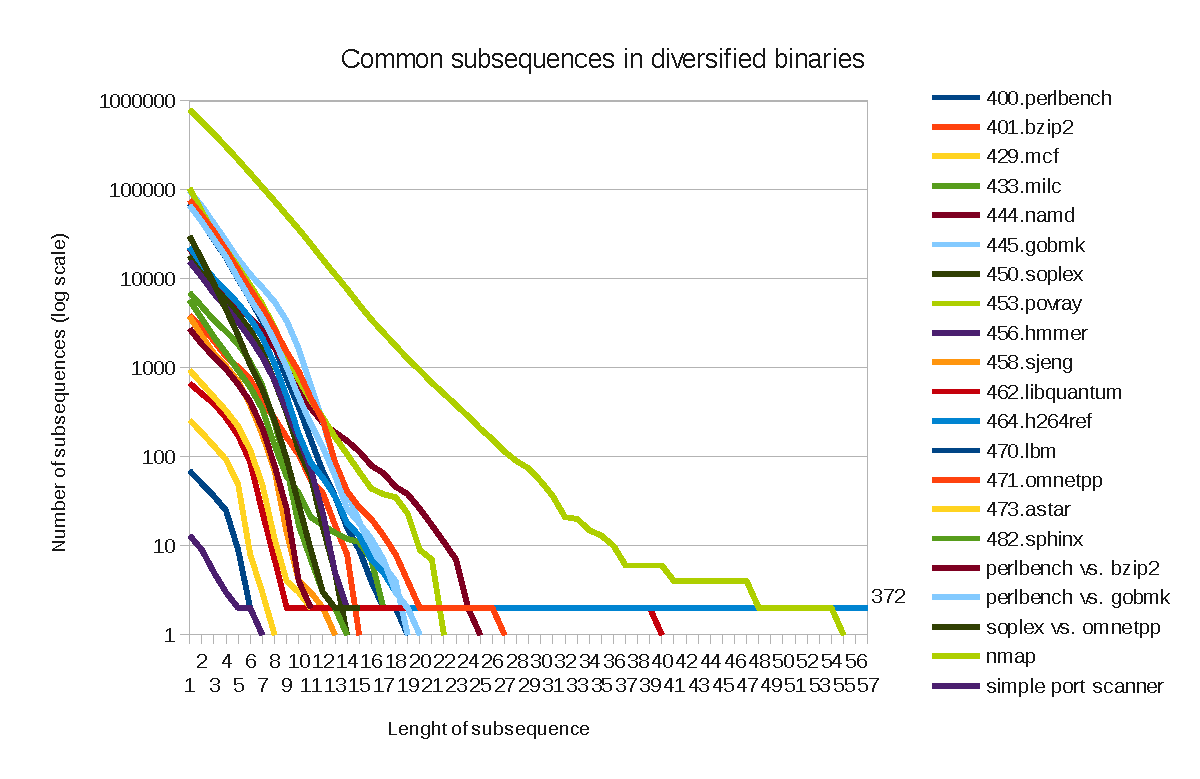
\includegraphics[width=85mm]{figures/subsequences-spec}
   \caption{List of common subsequences for SPEC CPU2006 benchmarks (log
     scale).}
   \label{fig:subsequencesspec}
 \end{center}
\end{figure}

\autoref{fig:subsequencesspec} shows (i) the list of SPEC benchmarks always
comparing two different diversified versions with each other, (ii) perlbench
compared with bzip and perlbench compared with gobmk to show the similarity
between two different programs, and (iii) two diversified versions of nmap and a
simple port scanner.

From \autoref{fig:subsequencesspec} we see that few shared substrings are longer
than 20 bytes of length and most shared substrings are shorter than 20 bytes.
The longer substrings all fall into one of the following criteria: start files
(shared among all programs compiled by the same compiler), function call
sequences (pushing parameters on to the stack), \texttt{mov} sequences (a set of
\texttt{mov} instructions that initialize structures), floating point sequences
that are currently not (yet) diversified, or hand written assembler
instructions. Of these substrings only the handwritten assembly instructions
pose a problem as they cannot be automatically broken up by the compiler. Apart
from these limitations it will be hard for malware analysts to come up with
efficient signatures for diversified binaries.


\subsection{Possible mitigation}

The evaluation showed that any signature-based matching is no longer effective
for diversified binaries. Combined with the high frequency in which diversified
binaries can be generated malware diversity allows malware authors to spread
fast and far without wide-spread detection (individual malware instances can
still be analyzed on a per-case basis).

Static and dynamic behavioral analysis of individual malware samples is of
course possible and will discover simple malware families. We assume that
malware authors will rely on existing anti-debugging and anti-forensics tools
to mitigate these risks. Anti-debugging and anti-forensics is orthogonal to
malware diversity and not part of MalDiv. Malware products will quickly
incorporate anti-debugging and anti-forensic measurements on their own.

Graph-based binary similarity analysis tools like bindiff can still effectively
recover some similarity between diversified instances due to the limited
diversification of the control-flow that is implemented in the current MalDiv
prototype. Bindiff shows reasonably high similarity between diversified
instances and reasonably low similarity between functionally different
binaries due to the differences in the control flow graph. Unfortunately,
bindiff has a very high analysis cost of up to 15 minutes to compare two
diversified instances. We reason that such a high analysis overhead will remain
unpractical for wide-spread deployment of such an analysis technique.


\section{Conclusion}\label{sec:concl}
%%%%%%%%%%%%%%%%%%%%%%%%%%%%%%%%%%%%%

Malware detection engines rely on signatures and common behavior to
successfully detect malware. The assumption of these detection mechanisms is
that each malware (family) can be classified using some form of signature.

In this paper we introduce malware diversity which breaks the above mentioned
assumption. Our prototype MalDiv, a malware diversification technique
automatically diversifies malware during the compilation. The LLVM-based
technique produces a large amount of binaries with very low similarity in a
short amount of time.

\acks

The idea to this project originates from a discussion between Stefan Brunthaler,
Per Larsen, and Mathias Payer. The work presented here (ab)uses all the great
multicompiler~\cite{multicompiler} work of Michael Franz's group to maximize the
differences between produced binaries and to minimize similarity according to
different metrics and adds a data diversification module for static data. This
project builds on a lot of feedback, great discussions, and help from Michael
Franz, Stefan Brunthaler, Per Larsen, Richard Wartell, and Stephen Crane.

%Acknowledgments, if needed.

% We recommend abbrvnat bibliography style.
{%\footnotesize
\linespread{0.85}
\bibliographystyle{abbrvnat}
\bibliography{bibliography}
}

\end{document}
